\documentclass[a4paper]{article}
\usepackage[14pt]{extsizes} 
\usepackage[T2A]{fontenc}
\usepackage[utf8]{inputenc}
\usepackage{natbib}
\usepackage{graphicx}
\usepackage{amsmath}
\usepackage[english]{babel}
\usepackage{fontspec}
\usepackage{amsmath,amsfonts,amssymb,amsthm,mathtools,mathrsfs}
\usepackage{icomma}
\usepackage{fullpage}
\usepackage{ulem}
\usepackage{eufrak}
\usepackage{setspace}
\usepackage{listings}
\usepackage{indentfirst}
\usepackage[left=2cm,right=1.5cm,top=2cm,bottom=2cm]{geometry}
\usepackage{xcolor}
\usepackage{float}
\usepackage{csquotes}

\setmainfont[Ligatures={TeX,Historic}]{Times New Roman}
\setlength{\parindent}{5ex}
\setlength{\parskip}{1em}
\renewcommand{\baselinestretch}{1}

\graphicspath{{images/}}

\definecolor{buzzlightyear}{HTML}{8757A5}
\definecolor{grass}{HTML}{738D06}
\definecolor{literal}{HTML}{F18A2B}
\definecolor{commentcolor}{HTML}{8E908B}

\lstdefinestyle{habrstyle}{
    backgroundcolor=\color{white},   
    commentstyle=\color{commentcolor},
    keywordstyle=\bfseries\color{buzzlightyear},
    numberstyle=\tiny\color{commentcolor},
    stringstyle=\color{grass},
    basicstyle=\ttfamily\footnotesize,
    breakatwhitespace=false,         
    breaklines=true,                 
    captionpos=b,                    
    keepspaces=true,                 
    numbers=left,                    
    numbersep=5pt,                  
    showspaces=false,                
    showstringspaces=false,
    showtabs=false,                  
    tabsize=4
}

\lstset{style=habrstyle}

\begin{document}

    % FIRST PAGE
    \begin{center}
        \begin{center}
        \hfill \break
        \normalsize{Санкт-Петербургский государственный политехнический}\\
        \normalsize{университет Петра Великого}\\
        \hfill \break
        \normalsize{\textbf{Высшая школа интеллектуальных систем и}}\\ 
        \normalsize{\textbf{суперкомпьютерных технологий}}\\ 
        \hfill \break
        \hfill \break
        \hfill \break
        \normalsize{Лабораторная работа}\\
        \hfill \break
        \hfill \break
        \normalsize{\LARGE Сигналы и звуки}\\
        \end{center}
        \hfill \break
        \hfill \break
        \hfill \break
        \hfill \break
        \hfill \break
        \hfill \break
        \hfill \break
        \hfill \break
        \hfill \break
        \hfill \break
        \begin{flushright}
            \normalsize{Работу выполнил студент}\\
            \normalsize{3-го курса, группа 3530901/80201}\\
            \normalsize{Сахибгареев Рамис Ринатович}\\
            \hfill \break
            \normalsize{Преподаватель:}\\
            \normalsize{Богач Наталья Владимировна}\\
        \end{flushright}
        \hfill \break
        \hfill \break
        \hfill \break
        \hfill \break
        \begin{center} Санкт-Петербург 2021 \end{center}
        \thispagestyle{empty}
    \end{center}
    % FIRST PAGE [END]
    
    \newpage
        \tableofcontents
    
    \newpage
         \listoffigures
    
    \newpage
         \lstlistoflistings   
     
    % START START START START START
    \newpage
        \section{Part 1: Check}
        
        In this part we need to make sure, that every listing is able to be executed. To do it, we can simply try to execute every example.
        
        After executing every input in "chap1" file no problems was found (Figure \ref{fig:work_check}).
        
        \begin{figure}[h]
            \centering
            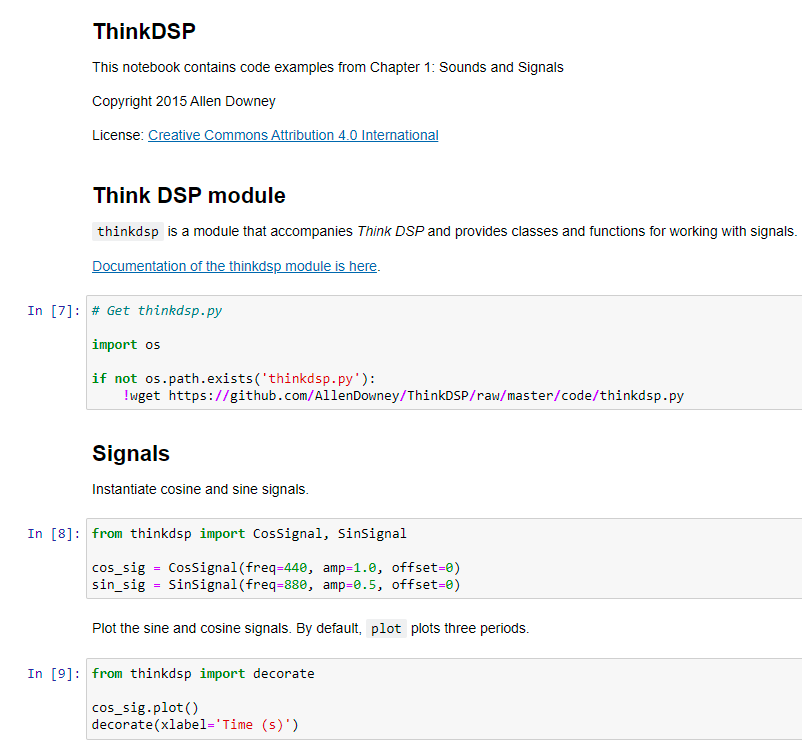
\includegraphics[width=\textwidth]{img/check.png}
            \caption{Everything is working fine}
            \label{fig:work_check}
        \end{figure}
    
    \newpage
        \section{Part 2: Processing}

        In this part we need to download any sound, that contains a clear pitch. Halzion by YOASOBI
        was selected. We need to select a half second interval with consistent pitch level, compute its spectrum. After harmonic filtration should be performed and spectrum should be converted back to the wave.
        
        Firstly we need to import required libraries to the project (Listing \ref{lst:imports_part_2})
            
        \begin{lstlisting}[language=Python,caption={Libraries import},label={lst:imports_part_2}]
            import os
            if not os.path.exists('thinkdsp.py'):
                !wget https://github.com/AllenDowney/ThinkDSP/raw/master/code/thinkdsp.py
            from thinkdsp import read_wave
            from thinkdsp import decorate
        \end{lstlisting}
        
        After imports done we can easily create a wave of the .wav file (Listing \ref{lst:halzion_to_wave}). Plot of the wave looks in the next way (Figure \ref{fig:halzion_wave_plot}).
            
        \begin{lstlisting}[language=Python,caption=Wav file conversion to wave instance,label={lst:halzion_to_wave}]
            wave = read_wave('sound/halzion.wav')
            wave.normalize()
            wave.make_audio()
        \end{lstlisting}

        \begin{figure}[H]
          \centering
          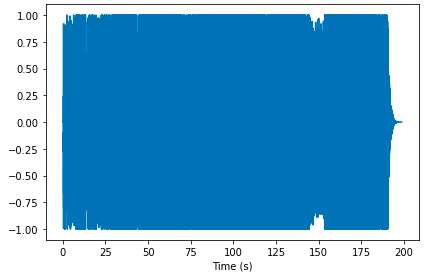
\includegraphics[width=\textwidth]{img/halzion_wave.png}
          \caption{Halzion's wave's plot}
          \label{fig:halzion_wave_plot}
        \end{figure}
            
        Selected half second segment starts at 1:42 (Listing \ref{lst:halzion_seg_ext}).
            
        \begin{lstlisting}[language=Python,caption=Segment extraction,label={lst:halzion_seg_ext}]
            segment = wave.segment(start=102, duration=0.5)
            segment.make_audio()
        \end{lstlisting}

        Using \texttt{segment.plot} next plot was acquired (Figure \ref{fig:segment_plot}). Spectrum was acquired using next functions (Listing \ref{lst:seg_spec_ext}). Spectrum of the segment can be viewed on the Figure \ref{fig:seg_spec_plot}.
            
        \begin{figure}[H]
            \centering
            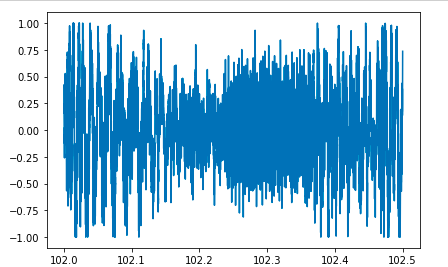
\includegraphics[width=\textwidth]{img/seg_wave.png}
            \caption{Segment's plot}
            \label{fig:segment_plot}
        \end{figure}
            
        \begin{lstlisting}[language=Python,caption=Segment spectrum calculation,label={lst:seg_spec_ext}]
            spectrum = segment.make_spectrum()
            spectrum.plot()
            decorate(xlabel='Frequency (Hz)')
        \end{lstlisting}

        \begin{figure}[H]
            \centering
            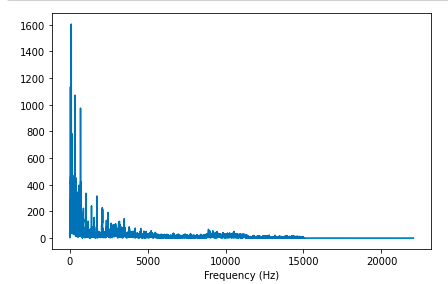
\includegraphics[width=\textwidth]{img/seg_spec.png}
            \caption{Segment's spectrum}
            \label{fig:seg_spec_plot}
        \end{figure}
            
        We can see, that higher frequencies are unused, so we can zoom in more dense area between 0 Hz and 5000 Hz (Figure \ref{fig:seg_spec_zoom}). We can clearly see spikes on the plot.
            
        \begin{figure}[H]
            \centering
            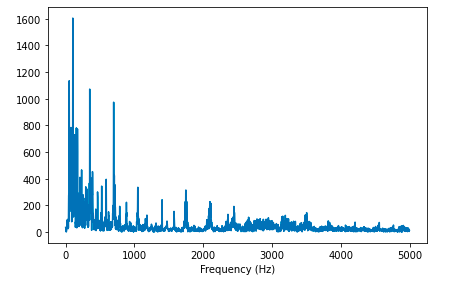
\includegraphics[width=\textwidth]{img/seg_spec_zoom.png}
            \caption{Spectrum zoom in}
            \label{fig:seg_spec_zoom}
        \end{figure}
            
        To filtrate spectrum next code Listing \ref{lst:spec_filt} was used. Result can be observed on the Figure \ref{fig:filt_wave_plot}.
        
        \begin{lstlisting}[language=Python,caption=Spectrum filtering,label={lst:spec_filt}]
            filtered = spectrum.high_pass(cutoff=500, factor=0.5)
            filtered = spectrum.make_wave()
            filtered.normalize()
            filtered.plot()
            decorate(xlabel='Time (s)')
        \end{lstlisting}
        
        \begin{figure}[H]
            \centering
            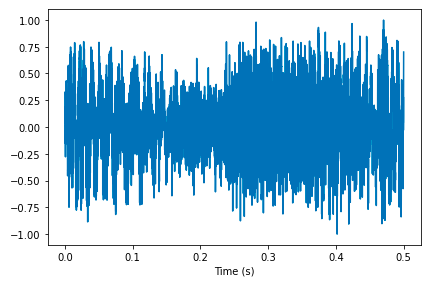
\includegraphics[width=\textwidth]{img/spec_filt_wave.png}
            \caption{Filtered spectrum's wave plot}
            \label{fig:filt_wave_plot}
        \end{figure}
        
        After listening filtered sound no differences was found, but background sounds became quieter.
        
    \newpage
        \section{Part 3: Combining}
            
        In this part we need to create 2 signals by summing a sine wave signal and a cosine wave signal. This signal should be converted to an audio and to a spectrum.
        
        Two signals was created. One with frequency of 555 Hz and other with frequency of 742 Hz (Listing \ref{lst:cos_sin_creat}). Result can be observed on the Figure \ref{fig:cos_sin_wave}.
            
        \begin{lstlisting}[language=Python,caption=Signal creation,label={lst:cos_sin_creat}]
            from thinkdsp import CosSignal , SinSignal
            cos_sig = CosSignal(freq=555, amp=0.82)
            sin_sig = SinSignal(freq=742, amp=0.42)
            cos_sig.plot()
            sin_sig.plot()
            decorate(xlabel='Time (s)')
        \end{lstlisting}
            
        \begin{figure}[H]
            \centering
            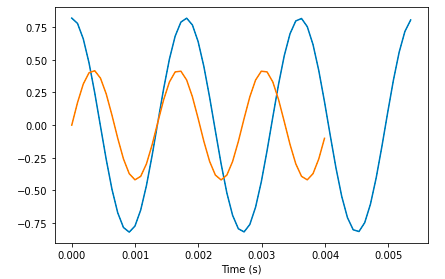
\includegraphics[width=\textwidth]{img/cos_sin.png}
            \caption{Created signals}
            \label{fig:cos_sin_wave}
        \end{figure}
            
        By summing them (Listing \ref{lst:cos_sin_summing}) next result was achieved (Figure \ref{fig:cos_sin_comb_wave}).
            
        \begin{lstlisting}[language=Python,caption=Summing the signals,label={lst:cos_sin_summing}]
            signal = cos_sig + sin_sig
            signal.plot()
            decorate(xlabel='Time (s)')
        \end{lstlisting}
            
        \begin{figure}[H]
            \centering
            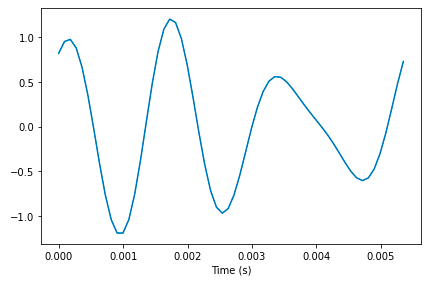
\includegraphics[width=\textwidth]{img/cos_sin_sum.png}
            \caption{Summing the signals}
            \label{fig:cos_sin_comb_wave}
        \end{figure}
        
        
            
        Wave and spectrum was created out of the signal using next code Listing \ref{lst:cos_sin_wave_creat}. Computed spectrum is next: Figure \ref{fig:cos_sin_spec}. We can clearly see 2 spikes with the frequencies of 555 and 742 Hz.
            
        \begin{lstlisting}[language=Python,caption=Creating a wave and a spectrum,label={lst:cos_sin_wave_creat}]
            sig_wave = signal.make_wave(duration = 10, start = 0, framerate = 400000)
            sig_spectrum = sig_wave.make_spectrum()
            sig_spectrum.plot(high=1000)
            decorate(xlabel='Frequency (Hz)')
        \end{lstlisting}    
            
         \begin{figure}[H]
            \centering
            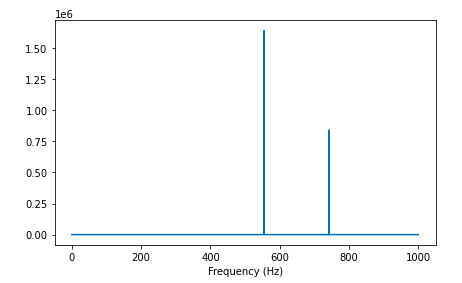
\includegraphics[width=\textwidth]{img/cos_sin_spec.png}
            \caption{Spectrum of combined signals}
            \label{fig:cos_sin_spec}
        \end{figure}
            
        By adding another signal to the existing one we are adding a new spile to the spectrum: Figure \ref{fig:cos_sin_new_sig}
        
        \begin{figure}[H]
            \centering
            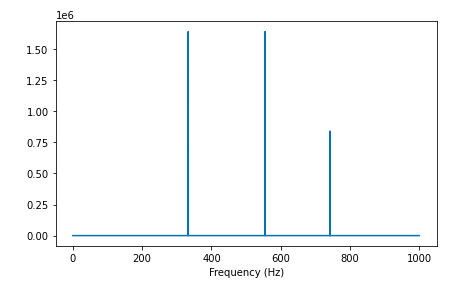
\includegraphics[width=\textwidth]{img/cos_sin_new_sig.png}
            \caption{Spectrum with one more added signal}
            \label{fig:cos_sin_new_sig}
        \end{figure}
            
        By adding low frequency signal, the sound became more flat and pleasant.
            
    \newpage
        \section{Part 4: Stretch}
        
            In this part we need to create function \texttt{stretch} to slow down or speed up the input wave by changing its \texttt{ts} and \texttt{framerate}.
            
            Code of the function is next: Listing \ref{lst:stretch_fun}
            
            \begin{lstlisting}[language=Python,caption=Definition of the function,label={lst:stretch_fun}]
                def stretch(wave, factor):
                wave.ts *= factor
                wave.framerate /= factor
            \end{lstlisting}
            
            Let's speed up YOASOBI's song by 20 percent (Figure \ref{fig:stretch_audio_res}). Original sound's length is 3:18, after stretching we've got 2:38.
            
            \begin{figure}[H]
                \centering
                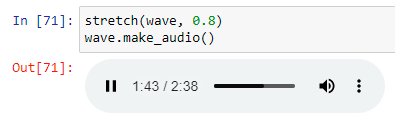
\includegraphics[width=\textwidth]{img/stretch_result.png}
                \caption{Function call result}
                \label{fig:stretch_audio_res}
            \end{figure}
    
    \newpage
        \section{Conclusion}
            Basic skills and knowledge of signals, waves and spectrum was acquired. Every signal can be decomposed into the set of frequencies and amplitudes of sine signal, that represents input signal. That allows to perform different operations on the signal, transport and store it.
            
            
    
\end{document}
